\documentclass[12pt]{article}
% Author: Luan Leal
% Last update: 2024-12-03

% ----------------------------

% ----------------------------   IMPORTS   ----------------------------
\usepackage{amssymb, amsthm, amsmath, geometry, siunitx, caption, float, graphicx}
\usepackage{enumitem}
\usepackage[utf8]{inputenc}
\usepackage[onehalfspacing]{setspaceenhanced}
\usepackage[brazil]{babel} % Adaptação ao pt-br
\usepackage{hyperref} % Usado para inserir links
\usepackage[capitalize, brazilian, noabbrev]{cleveref} % Referência adaptada ao pt-br
\usepackage{subcaption}
\usepackage{makecell}
\usepackage[num,overcite]{abntex2cite}

% ----------------------------   LAYOUT   ----------------------------
\citebrackets[]
\geometry{a4paper, lmargin=3cm, tmargin=3cm, rmargin=2cm, bmargin=2cm}
\onehalfspacing
%\setlength{\parindent}{45pt}
\sisetup{output-decimal-marker = {,}}

% ----------------------------  THEOREMS  ----------------------------
% -Ambiente de definição
\theoremstyle{definition}
\newtheorem{dfn}{Definição}[section]

% -Ambiente de observação
\theoremstyle{remark}
\newtheorem{obs}{Observação}

% -Ambiente de lema
\theoremstyle{definition}
\newtheorem{lema}{Lema}

% -Ambiente de exemplo
\theoremstyle{definition}
\newtheorem{xp}{Exemplo}[section]

% -Ambiente de proposição
\newtheorem{prop}{Proposição}

% -Ambiente de teorema e demonstração
\theoremstyle{plain}
\newtheorem{thm}{Teorema}
\theoremstyle{remark}
\newtheorem*{dms}{Demonstração}

% -Ambiente de exercício e resolução
\theoremstyle{definition}
\newtheorem{xcs}{Exercício}
\theoremstyle{remark}
\newtheorem*{rsl}{Resolução}

% ----------------------------  COMMANDS  ----------------------------
%\newcommand{\RR}{\mathbb{R}} % \mathbb{R} = \RR
%\newcommand{\ZZ}{\mathbb{Z}} % \mathbb{Z} = \ZZ

\author{Luan Leal (15470820); Micael Baruch (15578823)}
\captionsetup{margin=10pt,font=small,labelfont=bf,labelsep=period}
\usepackage{wrapfig}
\renewcommand{\baselinestretch}{1.5}

\title{Relatório - Seção A}

\begin{document}
\maketitle

    %Colocar um resumo?
    
    \begin{abstract}

    A leishmaniose é uma doença infecciosa causada por protozoários do gênero
    \textit{Leishmania}, transmitidos pela picada de flebotomíneos. Suas
    manifestações clínicas variam de formas cutâneas autolimitadas a formas
    viscerais graves e potencialmente fatais. O diagnóstico precoce e preciso é
    fundamental para o manejo clínico eficaz e o controle epidemiológico da
    doença. Dentre os métodos diagnósticos disponíveis, as técnicas moleculares
    têm se destacado pela elevada sensibilidade e especificidade, especialmente
    aquelas baseadas na extração e análise do DNA do parasita. Neste estudo,
    aplicaram-se métodos moleculares para verificar a presença de
    \textit{Leishmania} em uma amostra-problema (W) e, em caso positivo,
    determinar a espécie envolvida. O DNA extraído apresentou alta pureza
    (A\textsubscript{260}/A\textsubscript{280} = 2{,}07;
    A\textsubscript{260}/A\textsubscript{230} = \num{2.31}) e
    concentração adequada (\qty{140.1}{\nano\gram\per\micro\liter}), sendo
    amplificado com sucesso por PCR. A eletroforese em gel de agarose revelou um
    fragmento compatível com o tamanho esperado, indicando a presença do
    patógeno. Adicionalmente, a análise por qPCR com \textit{High Resolution
    Melting} (HRM) corroborou os resultados obtidos, permitindo a diferenciação
    entre espécies do complexo \textit{Leishmania spp.}. A amostra W apresentou
    perfil de fusão compatível com \textit{Leishmania amazonensis}, confirmando
    a eficácia e robustez da abordagem molecular empregada para o diagnóstico
    específico da leishmaniose. 

\end{abstract}

    \section{Introdução}
%TODO: Adicionar descrição dos métodos na contextualização
%TODO: Adicionar explicação da sigla PCR na contextualização
%TODO: Remover subseções 
%TODO: mover objetivos para o final

Leishmanioses são doenças infecciosas causadas por protozoários do gênero
\textit{Leishmania}, transmitidos por flebotomíneos e endêmicos em 98 países,
afetando mais de 350 milhões de pessoas\cite{hong2020one}. Essas doenças
apresentam manifestações clínicas diversas — de lesões cutâneas autolimitadas à
leishmaniose visceral fatal — que variam conforme a espécie envolvida. No
entanto, a diversidade de espécies causadoras de leishmanioses e as semelhanças
nos sintomas apresentados entre elas dificulta o adequado tratamento
espécies-específico da doença.

A complexidade da epidemiologia da leishmaniose demanda ferramentas diagnósticas
precisas, rápidas e economicamente viáveis.  Neste cenário, métodos moleculares
podem ser a chave na identificação da espécie de \textit{Leishmania} envolvida
na infecção. O presente trabalho teve como objetivo reproduzir de forma adaptada
os métodos moleculares de Graça
et.al.\cite{RFLPgraca2012} e Zampieri et.al.\cite{HRMzampi2016} com objetivo de
diagnosticar dentre as espécies \textit{Leishmania (Leishmania) infantum},
\textit{Leishmania (Leishmania) amazonensis}, \textit{Leishmania (Viannia)
braziliensis} e \textit{Leishmania (Viannia)
shawi} em uma amostra de DNA desconhecida. 

\subsection{Espectrofotometria, Eletroforese e PCR-RFLP}

A espectrofotometria por NanoDrop é uma técnica amplamente utilizada para avaliar a pureza e a 
concentração de ácidos nucleicos extraídos. A quantificação é realizada por meio da absorbância da 
amostra em diferentes comprimentos de onda, especialmente em \SI{260}{\nano\meter} para DNA e RNA, 
e em \SI{280}{\nano\meter} para proteínas. As razões A\textsubscript{260}/A\textsubscript{280} e A\textsubscript{260}/A\textsubscript{230} permitem 
inferir o grau de pureza do material, sendo valores entre 1{,}8 e 2{,}0 indicativos de DNA livre de proteínas 
e valores acima de 2{,}0 livre de outros contaminantes orgânicos~\cite{nanodrop}. Além disso, a pequena quantidade de amostra requerida (1–2~\si{\micro\liter}) 
torna o NanoDrop uma ferramenta rápida e eficiente para controle de qualidade de extrações de DNA antes de análises subsequentes.
% A métrica dada pelas professoras foram essas, porém nos artigos só encontro que A260/A280 ~ 1,8-2,0 e A260/A260 ~ 2,0-2,2

A eletroforese em gel de agarose é um método essencial para a visualização e separação de fragmentos de DNA com base em seu tamanho. 
Após a aplicação das amostras em poços de um gel de agarose e aplicação de corrente elétrica, os fragmentos de DNA migram em direção 
ao polo positivo. A velocidade de migração depende do tamanho dos fragmentos — quanto menor o fragmento, maior sua mobilidade. 
A adição de agentes intercalantes, como brometo de etídio ou SYBR Safe, permite a visualização das bandas de DNA sob luz ultravioleta. 
Esta técnica permite confirmar o sucesso de amplificações por PCR, avaliar a integridade do DNA e estimar o tamanho dos amplicons 
com base em marcadores de peso molecular~\cite{costa1998leishmaniose}.

A PCR seguida de análise por polimorfismo de fragmento de restrição (PCR-RFLP) é uma técnica molecular que combina amplificação de regiões 
específicas do DNA com digestão enzimática, visando identificar variações na sequência por meio do padrão de fragmentos gerados. Inicialmente, 
uma região alvo do genoma é amplificada por PCR. Em seguida, a amostra é incubada com enzimas de restrição que reconhecem sequências específicas 
de nucleotídeos. Alterações pontuais no DNA — como SNPs — podem criar ou abolir locais de corte, resultando em perfis distintos de bandas após separação 
por eletroforese em gel. A PCR-RFLP é especialmente útil para diferenciação de espécies, genotipagem e identificação de variantes alélicas, sendo 
considerada uma técnica de baixo custo, reprodutível e aplicável em diferentes contextos epidemiológicos e diagnósticos~\cite{garcia2005metodos}.

\subsection{qPCR e HRM}
A PCR em tempo real (qPCR)  é um método molecular baseado na amplificação da
quantidade de fitas de DNA por ciclos, enquanto a fluorescência emitida por
corantes intercalantes, é monitorada em tempo real a cada ciclo de amplificação.
Como o aumento da fluorescência é proporcional à quantidade de DNA amplificado,
torna-se possível quantificar o material genético na amostra\cite{Galluzi2018}.
A qPCR associada a análise \textit{High Resolution Melting} (HRM) implica que
após a amplificação, é realizada uma análise de dissociação da dupla fita com
relação à temperatura (\textit{melting curve}). Para tanto, a temperatura é
elevada gradualmente, à um passo definido e a fluorescência é medida
continuamente. À medida que as duplas fitas de DNA se dissociam em fitas
simples, a fluorescência diminui bruscamente, gerando uma curva característica
de cada amplicon. Isto permite a detecção de variações sutis na sequência de DNA
— como polimorfismos de nucleotídeo único (SNPs), inserções, deleções ou
diferenças no conteúdo de GC — por meio de alterações no formato da curva e na
temperatura de melting (Tm)\cite{Wittwer2009} por consequência da natureza
termoquímica destas variações.

No contexto da leishmaniose, a qPCR-HRM tem grande potencial
para o diagnóstico molecular e a discriminação de espécies de
\textit{Leishmania}. Para tanto, a elaboração de primers específicos para uma
sequência conservada entre as espécies, porém com pequenas variações em alguns
nucleotídeos permite obter perfis distintos de Tm e
formas de curva de dissociação para cada espécie.
Estudos anteriores foram bem-sucedidos em diferenciar espécies com base em
diferenças de menos de \qty{1}{\celsius}, na Tm dos amplicons
avaliados\cite{Azam2024,HRMzampi2016,SaadiBenAoun2024}.
Essa abordagem permite diagnósticos rápidos, sem necessidade de sequenciamento,
e pode ser integrada a plataformas de PCR em tempo real já existentes,
representando uma alternativa sensível, específica e custo-efetiva para a
identificação de espécies de \textit{Leishmania}.
 

    \section{Metodologia}
\subsection{Diapasão em um tubo fechado}
O estudo dos harmônicos em tubos fechados foi conduzido utilizando um arranjo experimental composto por um tubo cilíndrico fechado em uma de suas extremidades, um reservatório de água com altura ajustável e um conjunto de diapasões calibrados com frequências de 256 Hz, 384 Hz e 512 Hz. O tubo foi parcialmente preenchido com água, permitindo a variação da coluna de ar em seu interior através do ajuste da altura do reservatório de água como representado na \cref{fig:diapasao}.

\begin{figure}[H]
    \centering
    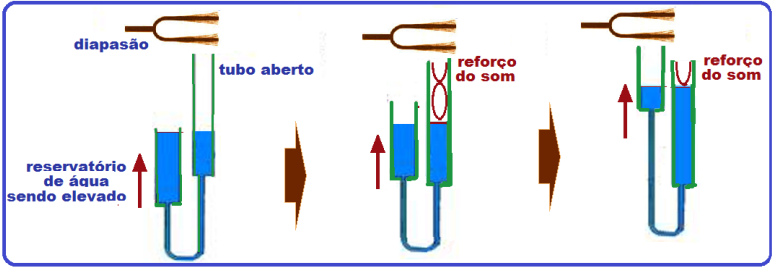
\includegraphics[width=0.50\linewidth]{fig/diapasao.png}
    \caption{Representação esquemática da montagem experimental para o estudo da ressonância em um tubo fechado. O tubo, com uma extremidade inferior fechada e parcialmente preenchido com água, permite ajustar a altura da coluna de ar por meio do nível da água, facilitando a identificação de harmônicos ao ser excitado por diapasões de diferentes frequências. Fonte: imagem fornecida pelo monitor Pedro.}
    \label{fig:diapasao}
\end{figure}

O procedimento experimental consistiu em excitar os diapasões e posicioná-los na abertura superior do tubo, perpendicularmente ao eixo longitudinal do mesmo. A altura da coluna de água foi ajustada sistematicamente até que a ressonância fosse observada.

\subsection{Ressonância e vibração em diapasão}
O arranjo experimental incluiu um diapasão de frequência fixa de 256 Hz e um segundo diapasão com frequência ajustável, equipado com um sistema de ímãs para calibração (\cref{fig:ressonancia}). A detecção da vibração no diapasão ajustável foi realizada utilizando uma pequena esfera de massa desprezível suspensa por um fio, que estava em contato com uma das hastes do diapasão.

\begin{figure}[H]
    \centering
    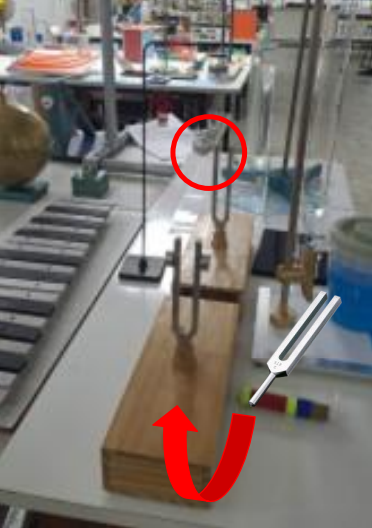
\includegraphics[width=0.25\linewidth]{fig/ressonacia.png}
    \caption{Fotografia do experimento de ressonância entre dois diapasões realizada no laboratório. O primeiro diapasão, circulado em vermelho, possui frequência fixa de 256 Hz, enquanto o segundo tem frequência ajustável por meio de ímãs. A vibração induzida é detectada por uma esfera suspensa em contato com uma das hastes do primeiro diapasão. Fonte: fotografia tirada pelo monitor Pedro}
    \label{fig:ressonancia}
\end{figure}

O procedimento iniciou-se com os dois diapasões já ajustados para a mesma frequência de 256 Hz. Em seguida, o diapasão de frequência ajustável foi percutido, e observou-se a esfera suspensa em contato com uma das hastes do primeiro diapasão. 

\subsection{Figuras de Chladni}
O estudo das figuras de Chladni foi realizado empregando duas placas metálicas planas, uma triangular e a outra quadrada, e um arco de violino (\cref{fig:chladni}). O procedimento experimental consistiu em aspergir uma fina camada de areia sobre a superfície da placa. Em seguida, a placa foi fixada em pontos estratégicos e excitada pela fricção do arco em suas bordas, gerando vibrações.

\begin{figure}[H]
    \centering
    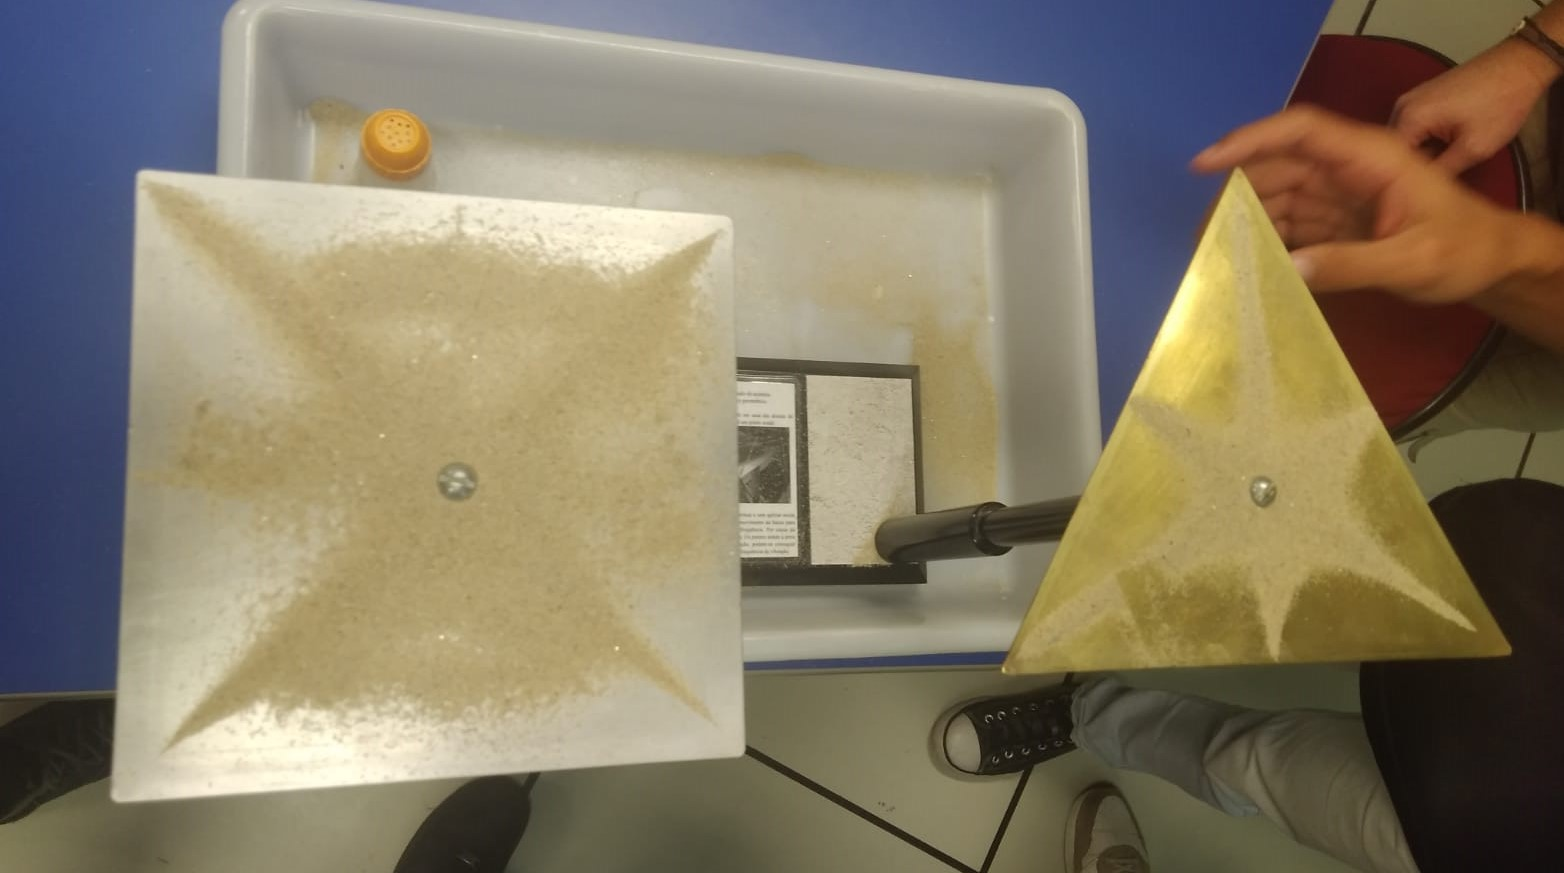
\includegraphics[width=0.35\linewidth]{fig/chladni.png.jpg}
    \caption{Fotografia tirada durante a realização do experimento de figuras de Chladni no laboratório. As placas metálicas de diferentes formas (quadrada e triangular) foram excitadas com um arco de violino, que não esta visível na imagem, formando padrões visíveis na superfície das placas. Fonte: autoria própria}
    \label{fig:chladni}
\end{figure}


Durante a experimentação, variaram-se os pontos de apoio da placa e os locais de aplicação da fricção do arco, permitindo a observação de diferentes padrões nodais formados pela areia. A análise qualitativa das figuras foi realizada para investigar a relação entre a geometria da placa, os pontos de excitação e as configurações dos padrões nodais.

\subsection{Tubo de Rijke}
O aparato experimental consistiu em um tubo cilíndrico aberto em ambas as extremidades e uma tela de malha metálica posicionada próxima a uma das extremidades do tubo. A fonte de calor de uma vela foi utilizada para aquecer a tela (\cref{fig:rijke}).

\begin{figure}[H]
    \centering
    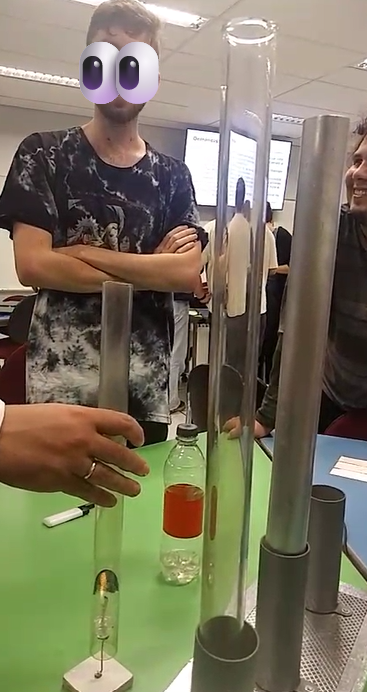
\includegraphics[width=0.25\linewidth]{fig/rijke.png}
    \caption{Registro fotográfico do experimento do tubo de Rijke feito em ambiente de laboratório. A malha metálica é aquecida por uma chama, gerando posteriormente uma emissão sonora característica quando o tubo é posicionado verticalmente. Fonte: autoria própria.}
    \label{fig:rijke}
\end{figure}

O procedimento envolveu o aquecimento inicial da tela metálica utilizando a chama da vela. Após um período de aquecimento, o tubo foi removido da chama e posicionado verticalmente. A emissão de um som característico foi observada. A influência da orientação do tubo (horizontal ou vertical) na emissão sonora foi qualitativamente investigada.

\subsection{Vibração de uma corda}
O estudo das vibrações em uma corda foi realizado utilizando um aparato que permitia variar a tensão e o comprimento efetivo da corda. O sistema incluía uma corda tensionada entre dois pontos fixos, sendo um deles móvel para ajustar o comprimento, e um mecanismo de pesos para aplicar e mensurar a tensão como mostrado na \cref{fig:umacorda}.

\begin{figure}[H]
    \centering
    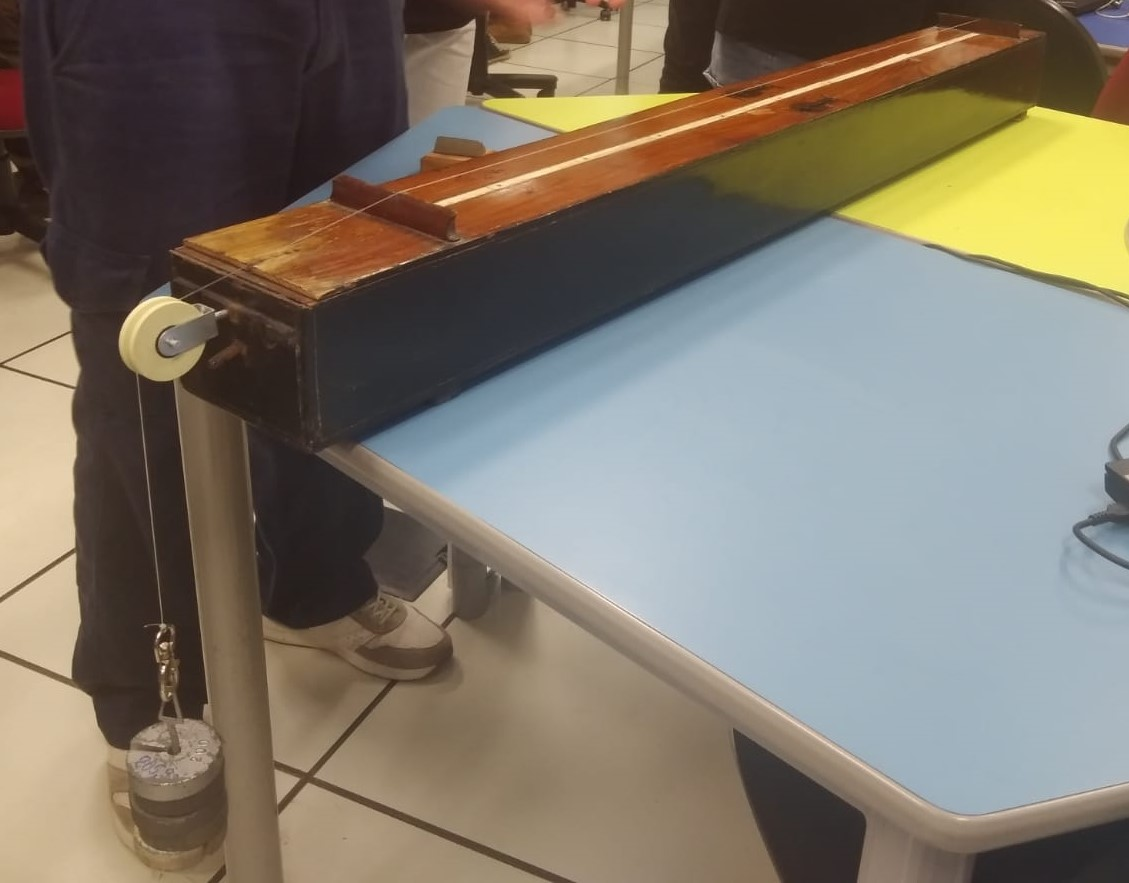
\includegraphics[width=0.30\linewidth]{fig/umacorda.png.jpg}
    \caption{Fotografia da montagem utilizada no laboratório para investigar os modos de vibração de uma corda tensionada. A tensão é aplicada com o uso de massas e o comprimento pode ser ajustado. Fonte: autoria própria.}
    \label{fig:umacorda}
\end{figure}

O experimento focou na observação dos sons gerados na corda e na relação entre a frequência de vibração, a tensão, o comprimento e a densidade linear da corda. A variação da tensão da corda e do seu comprimento efetivo foi realizada sistematicamente, e a resposta vibracional foi observada.
    \section{Resultados e discussões}

\subsection{Anel de Gravesande}
Ao realizar o experimento do Anel de Gravesande, observou-se que, à temperatura ambiente, a esfera metálica passava justamente através do anel. Após o aquecimento da esfera utilizando um pequeno balão cheio de álcool e com um pavio, notou-se que a esfera não conseguia mais atravessar o anel. Ao deixar a esfera esfriar por alguns instantes, ela voltava a passar pelo anel.

O funcionamento do Anel de Gravesande é uma demonstração clássica do fenômeno da dilatação térmica volumétrica dos sólidos. Em que quando um material é aquecido, a energia térmica fornecida aumenta a energia inética média de seus átomos e moléculas. Isso faz com que eles vibrem com maior amplitude, resultado em um aumento médio nas distancias interatômicas e, consequentemente, na expansão do volume do material.

Tal dilatação volumétrica (\(\Delta V\)) pode ser aproximada pela seguinte relação:
\begin{align*}
	\Delta V = V_0 * \gamma * \Delta T
\end{align*}
sendo, \(V_0\) o volume inicial do objeto, \(\gamma\) é o coeficiente de dilatação volumétrica do material e \(\Delta T\) é a variação de temperatura.

No caso do experimento realizado, a esfera era pequena, em uma ordem de, no máximo, uma dezena de centímetros, e o aquecimento da esfera, por ter sido realizado por pouco tempo e com uma pequena fonte de calor, a alteração de volume na esfera, foi de menos que um centímetro ao quadrado o que já foi o suficiente para impedir a passagem da esfera pelo anel.

Por fim, essa dinâmica física da dilatação térmica  volumétrica, é vastamente utilizada em diversas áreas da sociedade atual. Alguns exemplos mais práticos, é a utilização dessa dinâmica para a área industrial, para melhor encaixe de peças, e para a de resistência de alguns materiais, outro exemplo bem palpável é a utilização de termômetros de mercúrio, em que seu funcionamento se baseia na dilatação térmica do mercúrio em uma ampola graduada.  

\subsection{Par Bimetálico}
No experimento do par bimetálico, foi observado que, ao aquecer a lâmina bimetálica torcida, observou-se que a lâmina se esticava rapidamente, fazendo com que fosse puxado o ponteiro que estava na extremidade livre, assim fazendo-o movimentar e encostar na outra fase. Ao deixar a lâmina bimetálica esfriar por alguns instantes, observou-se que ela voltou à torção original, com o ponteiro para baixo, na fase inicial.

O funcionamento físico desse experimento do par bimetálico baseia-se na diferença do coeficiente de dilatação linear de dois metais distintos, que compõem a lâmina. Dessa forma, quando a lâmina é aquecida, ambos os metais tentam se expandir. No entanto, o metal com maior coeficiente de dilatação (\(\alpha_1\)) tenderá  a se expandir mais do que o metal com menor coeficiente de dilatação(\(\alpha_2\)) para a mesma variação de temperatura(\(\Delta T\)).

Como os dois metais estão unidos, eles não podem se expandir livremente de forma independente. Para acomodar essa diferença de expansão, a lâmina se curva para o lado que compõe o metal que possui o menor coeficiente de dilatação linear. Dessa forma, como a lamina estava enrolada, e ao aquecê-la, observou-se uma diminuição na torção, é possível dizer que a composição da lamina bimetálica tinha o metal com maior coeficiente de dilatação para fora, mostrado com a cor azul na Figura \cref{ParBimetalico}

\begin{figure}[H]
	\centering
	\includegraphics[width=0.25\linewidth]{fig/ParBimetálico.png}
	\caption{Lâmina bimetálica fixa composta por dois metais, representados pelas cores azul e vermelho, e ponteiro representado com verde. Fonte: Autoria própria.}
	\label{ParBimetalico}
\end{figure}

A capacidade do par bimetálico de se curvar de forma previsível com as mudanças de temperatura o torna muito útil em diversas aplicações práticas. Seu uso mais conhecido é em termostatos, onde funciona para controlar a temperatura em sistemas de ar condicionado, aquecedores e refrigeradores. Além disso, essa deformação causada pelo calor é o princípio de funcionamento de termômetros analógicos e de disjuntores térmicos, que são essenciais para proteger circuitos elétricos contra o superaquecimento resultante de correntes excessivas.

\subsection{Termoscópio}

Ao segurar o bulbo inferior de termoscópio, foi possível observar o nível da água subir pelo tubo. Similarmente, ao expor o termoscópio ao vento do ar condicionado da sala, foi possível observar o nível da água descer. Segurar o bulbo superior não causou modificação observável no termoscópio. A variação de temperatura observada é de aproximadamente \qty{10}{\celsius}, visto que a temperatura ambiente do dia era de aproximadamente \qty{25}{\celsius} e a temperatura da mão é de aproximadamente \qty{36}{\celsius}.  

A experiência é explicada pela variação de temperatura. Como o bulbo é de um vidro extremamente fino, ao segurar, a temperatura da mão e a temperatura do ar e da água no bulbo começam a entrar em equilíbrio. A mão, estando mais quente, transfere energia cinética para as moléculas de gás no bulbo na forma de calor. As moléculas de gás com maior energia cinética aumentam a intensidade média da força aplicada sobre a superfície de água. Isto é, há aumento de pressão sobre a superfície da água. Portanto, passa a existir uma diferença entre a pressão sobre a água fora do tubo e a pressão sobre a água dentro do tubo. Esta diferença de pressão resulta em uma força que gera o movimento da água para dentro do tubo. 

O contrário acontece quando expomos o tubo ao vento frio do ar condicionado. A cada instante de tempo, o ar mais frio remove energia cinética das moléculas de gás dentro do bulbo. Desta forma, a intensidade média da força com que as moléculas de gás atingem a superfícies da água diminui. Isto gera diferença de pressão entre a água dentro do tubo e a água fora do tubo. Esta diferença de pressão  tem como resultado a força que move a água para fora do tubo de volta para o bulbo.

É importante ressaltar que, enquanto a temperatura da água varia durante o experimento, um líquido não pode se expandir livremente. Ou seja, a ``dilatação'' do líquido não é suficiente para explicar o fenômeno, portanto o que é observado é de fato a variação da pressão do gás sobre o líquido resultante da variação da temperatura. 

O termoscópio permite observar variações de temperatura em um alcance que depende das proporções dos bulbos e do tubo. Esta limitação faz com que seja dificultoso tomar medidas de grandes variações de temperatura sem ter um equipamento de tamanho desconfortável. Além disso, a sensibilidade de um equipamento maior seria menor em relação ao tempo. Isto é, para um equipamento das proporções utilizadas neste experimento foi possível contemplar a variação da temperatura de forma relativamente rápida, porém, quanto maior o equipamento, mais tempo levaria para que a transmissão de calor fosse suficiente para observar mudanças notáveis. 

\subsection{Termômetro de Galileu}

Em teoria, os bonecos deveriam flutuar de acordo com a temperatura do líquido. No entanto, durante a experiência, todos os bonecos permaneceram no fundo do tubo. Cada boneco teve sua densidade calibrada para permanecer em um nível à depender da temperatura do líquido. A hipótese óbvia de que a temperatura era tal que os bonecos permaneceriam afundados é facilmente descartada por duas razões. A primeira é que a calibração nominal acusa que este cenário só deveria ocorrer para temperatura ambiente igual ou superior a \qty{28}{\celsius}, o dia em questão estava frio e esta temperatura não parece razoável. A segunda razão é que ao resfriar o tubo expondo-o ao ar do ar condicionado os bonecos permaneceram no fundo do tubo. Desta forma, torna-se mais provável que tenham sido descalibrados. É possível que exista algum dano físico nos bonecos que tenha feito com que trocassem matéria com o líquido ou ainda que não tenham sido calibrados para as temperaturas nominais indicadas na \cref{temps}.

\begin{figure}[ht]
    \centering
    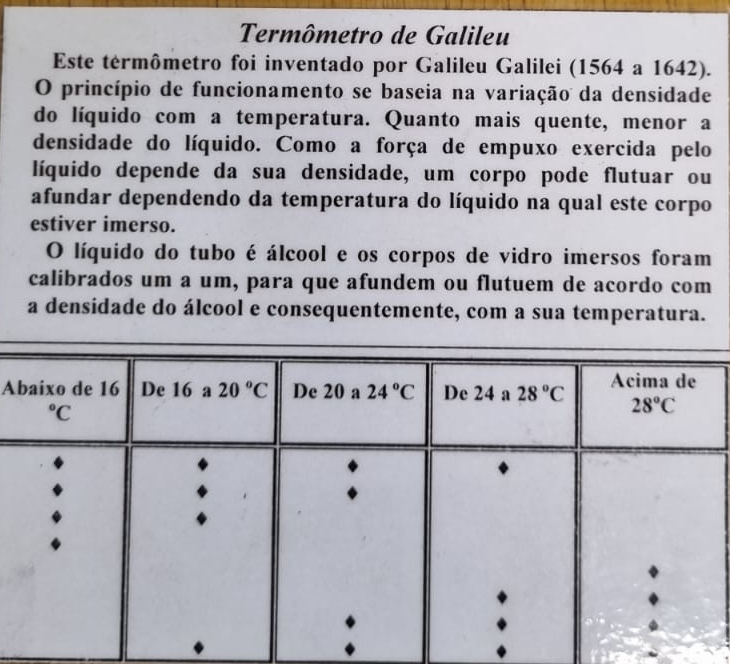
\includegraphics[width=.5\linewidth]{fig/temps}
    \caption{Temperaturas nominais e posições esperadas dos bonecos para cada uma}\label{temps}
\end{figure}

De toda forma, o princípio por trás deste experimento é a variação da densidade do líquido com a variação da temperatura. Ao aquecer, as moléculas que compõe o líquido têm maior energia cinética, aumentando, em média, a distância entre as moléculas do líquido. Desta forma, um objeto submerso no líquido está sujeito à força de empuxo deste, por sua vez, a força de empuxo varia com a densidade do líquido. Ao aumentar a temperatura a densidade do líquido diminui. Por consequência, aumento na temperatura resulta em diminuição da força de empuxo. Como os bonecos também estão sujeitos à força gravitacional, atuando sobre eles sem variação, na mesma direção e em sentido oposto ao da força de empuxo, ao diminuir a força de empuxo a força resultante se torna não nula e faz com que o boneco afunde um pouco mais. O contrário acontece ao resfriar o líquido. 

O termômetro de Galileu é um precursor engenhoso dos termômetros de mercúrio. Uma vantagem interessante deste em relação ao anterior é que não depende do uso de metais pesados. Porém, a resolução do termômetro de galileu depende de ajustar densidades muito próximas entre os objetos de medida, os bonecos no nosso caso. Além disso, o alcance de temperaturas mensuráveis com um termômetro de Galileu é limitado a variações de temperatura na escala da temperatura ambiente (\qty{10}{\celsius}--\qty{36}{\celsius}), não pode medir temperaturas próximas à temperatura de ebulição ou fusão do líquido utilizado. 

\subsection{Psicrômetro}
Foi constatado que o termômetro seco media \qty{25}{\celsius} e o termômetro molhado media aproximadamente \qty{22}{\celsius}. Ao consultar a tabela, temos que a diferença de temperatura é \qty{3}{\celsius}, portanto, umidade de \qty{76}{\percent} a \qty{77}{\percent} na sala. Durante este dia, a temperatura indicada pela previsão do tempo registrada no dia era de \qty{25}{\celsius} enquanto a umidade média no Butantã era de \qty{66}{\percent}. A diferença entre a umidade medida e a umidade média da região é provavelmente decorrente da arborização. Enquanto o campus da USP é bem arborizado e próximo ao rio Pinheiros e à raia, é de se esperar que seja uma região com pico de umidade do ar. 

O princípio por trás do psicrômetro é a termodinâmica. Em particular o equilíbrio de fases. Em todos os momentos, a água está sob pressão do vapor de água e sob agitação em decorrência da temperatura, portanto, o ponto de equilíbrio ocorre quando a pressão de vapor é tal que a quantidade de cada fase fique em equilíbrio dinâmico, o sistema tende à este ponto de equilíbrio. Pensando molecularmente, embora a temperatura seja uma medida da energia cinética média das moléculas de água a real distribuição da energia cinética é caótica e em determinados momentos há moléculas com mais energia cinética que as demais. Se a energia cinética de uma molécula é tal que supere a energia potencial que a atrai às outras moléculas de água, fazendo-a compor a fração líquida, então esta molécula pode se desprender e passar a compor a fração gasosa. 

Se a pressão de vapor for menor do que a pressão de equilíbrio para aquela temperatura, será recorrente que as moléculas se desprendam e evaporem sem condensar novamente. Durante o processo de evaporação, a água toma calor do termômetro, fazendo o medir temperatura mais fria do que o termômetro exposto ao ar. Como justificado, a variação da temperatura deve depender da umidade relativa do ar. Similarmente, se a concentração de moléculas de água no ar for tal que a pressão de vapor exercida sobre a gaze seja igual a pressão de vapor de equilíbrio, então não haverá evaporação e a diferença de temperatura será nula, indicando umidade relativa do ar de \qty{100}{\percent}. Ou seja, qualquer acréscimo de moléculas de água na fase gasosa resulta em condensação. Este é o mesmo fenômeno observado quando há formação de orvalho.

O psicrômetro de dois bulbos é prático por não depender de energia elétrica e ser fácil de carregar. Pode medir a umidade relativa de forma tão sensível quanto for a escala dos termômetros e da tabela. Visto que a pressão de vapor de equilíbrio pode ser determinada para cada temperatura. Como desvantagem, idealmente o psicrômetro é construído com água destilada para evitar variações no equilíbrio por composição química da água. Além disso, o alcance das medidas é limitado para temperaturas em que a água se mantenha líquida, dificultando utilizá-lo para medir umidade do ar em dias com temperaturas abaixo de zero. Por fim, é preciso manter a gaze sempre em contato com uma fonte de água destilada.


    \section{Discussão}
% TODO: Tirar toda a discussão dos resultados e passar pra cá -TF8

    \section{Conclusão} 
O Termoscópio de Galileu demonstrou eficazmente a expansão de gases mediante aquecimento e a consequente variação de pressão, evidenciada pelo deslocamento da coluna de água. Este experimento ilustrou um método qualitativo primordial para a detecção de variações de temperatura.

No estudo do Termômetro de Galileu, observou-se que os bulbos permaneceram submersos, contrariando a expectativa de flutuação diferencial conforme a temperatura. Tal resultado sugere uma possível descalibração do instrumento ou danos aos componentes, impedindo a demonstração prática do princípio da variação da densidade do líquido com a temperatura e seu efeito no empuxo.

O psicrômetro possibilitou a determinação da umidade relativa do ar por meio da diferença de temperatura entre um termômetro seco e um úmido, resultado da evaporação da água no bulbo deste último. A medição obtida foi contextualizada com dados meteorológicos regionais, destacando a influência de fatores locais como a vegetação.

O experimento com o Anel de Gravesande evidenciou o fenômeno da dilatação térmica em sólidos: a esfera metálica, que atravessava o anel à temperatura ambiente, não o fez após ser aquecida, voltando a passar após o resfriamento. Esta prática demonstrou como o aumento da temperatura leva à expansão volumétrica dos materiais.

Finalmente, o par bimetálico ilustrou a dilatação linear diferencial entre dois metais distintos. Ao ser aquecida, a lâmina bimetálica curvou-se devido à diferença nos coeficientes de dilatação dos seus componentes, um princípio fundamental em dispositivos como termostatos e disjuntores.


    \bibliography{refs}

\end{document}
